% !TeX spellcheck = de_DE
\section{Einf"uhrungsstrategien der Datenmigration}
\label{chapter:vorgehensweisen}
%TODO Julian
%http://www.information-management.com/specialreports/20040525/1003961-1.html
%http://edepositireland.ie/bitstream/handle/2262/27040/The%20Butterfly%20Methodology%20a%20gateway-free%20approach%20for%20migrating%20legacy%20information%20systems.pdf?sequence=1&isAllowed=y
%http://www.dtic.upf.edu/~jbisbal/publications/icsc97.pdf
%https://pure.fundp.ac.be/ws/files/168599/wcre02.pdf
%http://www.dtic.upf.edu/~jbisbal/publications/datasem97.pdf
%http://csis.pace.edu/~marchese/CS775/Proj1/legacyinfosys_directions.pdf

%Quellen hinzuf"ugen
% neue System -> Zielsystem + Definition?

Das vom Unternehmen angewandte Prozessmodell beinhaltet ebenso die Wahl einer Einf"uhrungsstrategie, welche den technischen Ablauf und die Einf"uhrung der Datenmigration beschreibt. Da die gew"ahlte Einf"uhrungsstrategie den weiteren Verlauf des Prozessmodells beeinflusst, wird diese in einer fr"uhen Phase, nachdem die Kerndaten von Legacy- und neuem System analysiert wurden, ausgew"ahlt. Eine sp"atere Revision dieser Entscheidung ist nicht oder nur sehr schwer m"oglich. Allerdings kann nicht jede Einf"uhrungsstrategie in jedem Kontext f"ur die Durchf"uhrung einer Datenmigration genutzt werden. Im Folgenden werden zu diesem Zweck drei Einf"uhrungsstrategien mit ihren jeweiligen Vor- und Nachteilen vorgestellt. 

\subsection{Big-Bang-Ansatz}

Der \textit{Big-Bang} oder auch als \textit{Cold Turkey} bekannte Ansatz ist wohl das "alteste Model zur Durchf"uhrung einer Datenmigration. Nachdem das Legacy- und das neue System ausreichend analysiert und deren Unterschiede bestimmt wurden, wird das Legacy-System abgeschaltet. Somit m"ussen s"amtliche vom Legacy-System gest"utzte Gesch"aftsprozesse unterbrochen werden \citep[S.~4]{wuLawless-1997}. 
\lb
W"ahrend dieser Unterbrechung wird ein \textit{Dump}\footnote{Ein \textit{Dump} (Auszug) ist ein Abbild des Speicherzustandes etwa einer Datenbank zu einem bestimmten Zeitpunkt} des gesamten Datenbestands des Legacy-Systems angelegt. Dieser wird anschlie"send mittels der hierf"ur entwickelten Migrationsskripte in das neue System "ubertragen \citep[S.~3]{brodie-1993}. Bis die Datenmigration abgeschlossen ist, "onnen weder das neue, noch das Legacy-System im Unternehmen eingesetzt werden. Hieraus resultiert ein Zeitraum, in welchem das Unternehmen auf kein lauff"ahiges System zur"uckgreifen kann und somit stark in seiner Gesch"aftsf"ahigkeit eingeschr"ankt ist \citep[S.~3f.]{brodie-1993}.
\lb
Die Vorteile diese Ansatzes beschr"anken sich auf das verbesserte Programmverst"andnis, die Performance und die bessere Wartbarkeit des neuen Systems. Nachteilig hingegen ist ein sehr hohes Risiko bei einem Scheitern der Einf"uhrung \citep[S.~105]{bisbal-1999}. Das hohe Risiko des Big-Bang-Ansatz besteht vor allem darin, dass der gesamte Datenbestand gesamtheitlich migriert wird. Eventuell auftretende Fehler k"onnen erst festgestellt werden, wenn die Datenmigration abgeschlossen ist. In diesem Fall muss der gesamte Prozess wiederholt werden. Neben dem hohen Risiko besteht bei Nutzung Big-Bang-Ansatzes ebenfalls der Nachteil der zeitweisen Unterbrechung aller vom Legacy- bzw. dem neuen System unterst"utzten Gesch"aftsprozesse, zum Zwecke der Durchf"uhrung der Datenmigration \citep[S.~4]{wuLawless-1997}.
\lb
Zusammenfassend bietet der Big-Bang-Ansatz auf der einen Seite eine unkomplizierte Datenmigration. Auf der anderen Seite jedoch stehen ein hohes Risiko bei der Einf"uhrung, sowie Ausfallzeiten w"ahrend der Einf"uhrung der "Anderungen. In diesem Zeitraum k"onnen Gesch"aftst"atigkeiten nur eingeschr"ankt oder gar nicht durchgef"uhrt werden. Der Big-Bang-Ansatz findet aufgrund des hohen Risikos in der heutigen Zeit sehr selten Anwendung in Unternehmen.

\subsection{Chicken-Little-Ansatz}

Der \textit{Chicken-Little}-Ansatz stellt eine weitere Einf"uhrungsstrategie zur Datenmigration dar. Entwickelt wurde dieser Ansatz von Michaell Brodie und Michael Stonebraker im Rahmen des 1991 begonnenen DARWIN-Projekts \citep{zoulafy-2002}. Der Chicken-Little-Ansatz ist im Gegensatz zum Big-Bang-Ansatz ein inkrementelles Vorgehen zur Datenmigration. Durch das inkrementelle Vorgehen sollen Schw"achen des Big-Bang-Ansatzes beseitigt werden. Es k"onnen durch den Chicken-Little-Ansatz etwa Ausfallzeiten der von Legacy- bzw. neuen System unterst"utzten Gesch"aftsprozesse w"ahrend der Datenmigration vermieden oder zumindest auf ein Minimum reduziert werden \citep{zoulafy-2002}.
\lb
Das inkrementelle Vorgehen erm"oglicht hierbei eine Entwicklung und Einf"uhrung aller "Anderungen im Rahmen kleinerer Module. Entwickelt und eingef"uhrt werden zun"achst wenige Anpassungen. Inkrementell k"onnen weitere Funktionalit"aten des Legacy-Systems und damit der migrierten Daten "ubertragen werden \citep[S.~2]{wuLawless-1997}.
\lb
Um auch w"ahrend der Datenmigration die kontinuierliche Arbeit mit Softwaresystemen zu erm"oglichen, kommt beim Chicken-Little-Ansatz ein sogenanntes \textit{Gateway} zum Einsatz. Dieses Gateway verbindet Legacy- und neues System nach "Anderung oder Neuentwicklung miteinander und koordiniert deren Kommunikation untereinander. Somit k"onnen das neue und das Legacy-System solange parallel ausgef"uhrt werden, bis das neue System alle Daten enth"alt und alle Funktionalit"aten "ubernehmen kann \citep[S.~2]{wuLawless-1997}. Die neuen Daten, welche innerhalb des Zeitraumes entstehen, in welchem das neue System noch nicht alle Funktionen "ubernommen hat, werden dabei auf dem f"ur diese Funktion zust"andigen System gespeichert. Folglich werden Daten, welche bereits durch das neue System erstellt worden sind auch dort gespeichert \citep[S.~2]{wuLawless-1997}. In gewissen Kontexten ist es sinnvoll, Daten zeitweise in beiden Systemen zu pflegen. Urspr"ungliche Schemata und Datenquellen werden erst verworfen, sobald zuk"unftige System diese Aufgaben verl"asslich erf"ullen k"onnen.
\lb
Das Gateway erf"ullt nun zwei Aufgaben beim "Ubertragen der Daten an das neue System. Zum einen ist dies das Bereitstellen der noch nicht migrierten Daten an das neue System. Zum Anderen das Bereitstellen der bereits migrierten Daten an das Legacy-System. Ersteres wird auch als umgekehrtes Gateway (engl.: \textit{reverse Gateway}) und letzteres als Vorw"arts-Gateway (engl.: \textit{forward Gateway}) bezeichnet \citep[S.~2]{wuLawless-1997}. Je nachdem, wie stark sich Datenbankschemata von Legacy- und neuem System unterscheiden, stellen vorw"arts- und umgekehrtes Gateway unterschiedlich komplexe Module dar. Mit steigender Komplexit"at dieser Module sinkt allerdings auch die Performance der Systeme w"ahrend der Migrationsphase \citep[S.~109]{bisbal-1999}.
\lb
"Ahnlich dem Big-Bang-Ansatz, bietet der Chicken-Little-Ansatz die erwarteten Verbesserungen in Performance, Wartbarkeit sowie im Verst"andnis des Systems \citep[S.~108]{bisbal-1999}. Allerdings fallen bei Einsatz des Chicken-Little-Ansatzes keine Ausfallzeiten, in denen weder mit Legacy- noch mit dem neuen System gearbeitet werden kann, an. Erm"oglicht wird dies durch den Einsatz des Gateways, wodurch auch w"ahrend der Migrationsphase mit dem gesamten System gearbeitet werden kann \citep[S.~2]{wuLawless-1997}. Dar"uber hinaus bietet der Chicken-Little-Ansatz noch weitere Vorteile. Es muss beispielsweise nicht das gesamte Legacy-System auf einmal ersetzt werden. Stattdessen kann dieses Modul f"ur Modul erneuert werden. Dies erleichtert Entwicklung bzw. Anpassung des neuen Systems \citep[S.~3]{brodie-1993}. Die inkrementelle Anpassung des neuen Systems bietet auch Vorteile in der Fehlerbehandlung. So m"ussen bei Auftreten von Fehlern nur die entsprechenden Schritte wiederholt werden. Wenn etwa ein Problem bei der Datenmigration eines entwickelten Moduls auftritt, muss nach der Fehlerbehebung lediglich die Datenmigration von diesem Modul wiederholt werden. Durch die Fehlerbehebung gewonnene Kenntnisse k"onnen ebenfalls in den n"achsten Schritten genutzt werden, um Probleme zu vermeiden, bevor diese entstehen \citep[S.~3]{brodie-1993}.
\lb
% je nach LIS unterschiedlich schwer durchzuf"uhren
Neben den genannten Vorteilen hat der Chicken-Little-Ansatz auch einige Nachteile aufzuweisen. Zwar erlaubt es der Einsatz eines Gateways, w"ahrend der Migrationsphase mit einem kombinierten System zu arbeiten, daf"ur stellt die Entwicklung des Gateway eine Herausforderung dar. Sie zieht unter Umst"anden hohe Kosten mit sich und erfordert eine hohes fachliches Verst"andnis beider Systeme. Daten, welche auf beiden Systemen vorhanden sind, m"ussen konsistent gehalten werden. Um die Interoperabilit"at der beiden Systeme zu erm"oglichen, muss das Gateway semantische und technische Verkn"upfungen beider Schemata herstellen. Je unterschiedlicher die Datenbankschemata von Legacy- und neuem System sind, desto komplexer erscheint diese Aufgabe \citep[S.~2f.]{wuLawless-1997}. Dar"uber hinaus muss bei komplexeren Gateways auch mit Einbu"sen im Hinblick auf Performance gerechnet werden, wenn ein vorw"arts- beziehungsweise umgekehrtes Gateway zum Einsatz kommt \citep[S.~109]{bisbal-1999}.
\lb
Alles in Allem betrachtet bietet der Chicken-Little-Ansatz viele Vorteile. Die inkrementelle Herangehensweise minimiert viele Risiken und Probleme, wie z.B. die Ausfallzeiten des Big-Bang-Ansatzes. Aus diesem Grund eignet sich Chicken-Little auch zum Einsatz in gr"o"seren Unternehmen. Jedoch muss bedacht werden, dass die Durchf"uhrung des Chicken-Little-Ansatzes dennoch sehr komplex erscheinen kann.

%\cleardoublepage

\subsection{Butterfly-Ansatz}

% versucht Problematik des Gateway zu umgehen
% Daten des Legacy-System werden in TempStorages "ubertragen
% Legacy-System bleibt bis Abschluss im Betrieb
% Nach "ubertragung der initialen Daten mittels temp0, wird temp1 mit den neuen Daten angelegt ...
% temp werden mit der Zeit immer kleiner bis temp so klein ist das dieses ausreichend schnell "ubertragen werden kann -> Abschalten des Legacy-System und abschließende "ubertragung
% minimal Downtime f"ur finale Daten"ubertragung bis das neue System eingesetzt werden kann

Im Rahmen des MILESTONE-Projektes von 1996 wurde in einer Kooperation des Trinity College Dublin, Broadcom \'{E}ireann Research, Telecom \'{E}ireann und Ericson der sogenannte \textit{Butterfly}-Ansatz entwickelt \citep[S.~202]{wuLawlessBisbal-1997}. Der Butterfly-Ansatz ben"otigt keine Gateways, die zwischen den Systemen vermitteln \citep[S.~202]{wuLawlessBisbal-1997}. Folglich ist es nicht m"oglich, dass w"ahrend der Datenmigration auf beiden Systemen gearbeitet werden kann. Allerdings ist diese Aussage nicht mit einer l"angeren Ausfallzeit, wie beim Big-Bang-Ansatz, gleichzusetzen. Stattdessen wird beim Butterfly-Ansatz mit tempor"aren Datenspeichern gearbeitet, welche die kontinuierliche Arbeit mit dem Legacy-System w"ahrend der Datenmigration erm"oglichen. Das neue System kommt erst zum Einsatz, sobald alle Daten auf dieses "ubertragen worden sind. Bis dies geschehen ist, bleibt das Legacy-System im Einsatz \citep[S.~3]{wuLawless-1997}.
\lb
Zu Beginn der Datenmigration wird beim Butterfly-Ansatz der aktuelle Datenbestand des Legacy-Systems eingefroren. Ab diesem Zeitpunkt k"onnen auf dem Legacy Datenbestand nur noch Lese-Aktionen durchgef"uhrt werden, jedoch k"onnen dort keine neuen Daten mehr hinterlegt werden \citep[S.~202]{wuLawlessBisbal-1997}. Um dennoch mit dem Legacy-System weiterarbeiten zu k"onnen, bedient sich der Butterfly-Ansatz eines tempor"aren Speichers sowie eines \textit{Data-Access-Allocator} (DAA). Dieser Data-Access-Allocator enth"alt Informationen dar"uber, wo welche Daten im eingefrorenen Datenbestand zu finden sind und welcher tempor"arer Speicher gerade aktiv ist \citep[S.~202]{wuLawlessBisbal-1997}. Wie Abbildung \ref{pic:datemigration_Butterfly} zeigt, wird der Data-Access-Allocator zwischen die Anwendungen und Dienste des Legacy-System und deren Datenbank geschaltet. Werden nun neue Daten ins Legacy-System eingegeben oder werden vorhandene bearbeitet, sorgt der Data-Access-Allocator daf"ur, dass die entsprechenden Daten aus dem eingefrorenen Datenbestand gelesen werden und neue Daten im aktuellen tempor"aren Speicher abgelegt werden \citep[S.~202]{wuLawlessBisbal-1997}.
\lb

\begin{figure*}[!t]
	\centering
	\caption{Datenmigration mittels des Butterfly-Ansatzes}
	\label{pic:datemigration_Butterfly}
	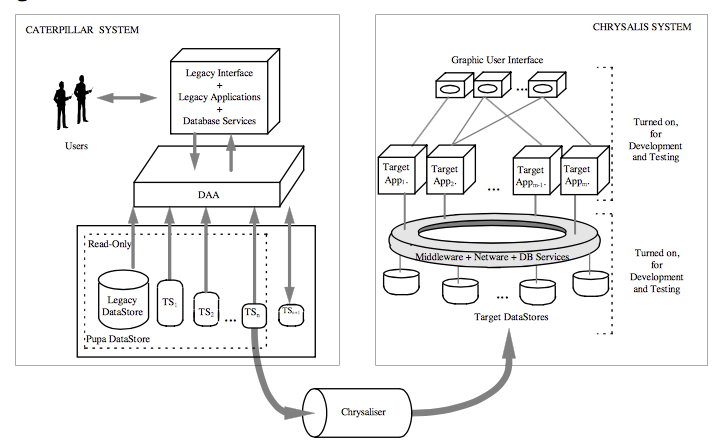
\includegraphics[width=1.0\textwidth]{../images/vorgehensweisen_fig_01.png} \\
	\small Quelle: \citep[Abbildung~11]{wuLawless-1997}
\end{figure*}

%\newpage

Durch Data-Access-Allocator und tempor"are Speicher wird sichergestellt, dass w"ahrend der Datenmigration mit dem Legacy-System normal weitergearbeitet werden kann. F"ur die "Ubertragung der Daten auf das neue System wird allerdings noch ein \textit{Daten-"-Transformator}, ein sogenannter \textit{Chrysaliser} ben"otigt \citep[S.~202]{wuLawlessBisbal-1997}. Dieser Chrysaliser "ubernimmt die Rolle der Migrationsskripte. Er enth"alt die Informationen "uber die Datenbankschemata des Legacy- und des neuen Systems sowie die Schemata des Legacy-Systems, welche umgewandelt werden m"ussen \citep[S.~202]{wuLawlessBisbal-1997}. 
\lb
Mit Hilfe des Chrysaliser werden nun die Daten aus dem eingefrorenen Datenbestand an das neue System "ubertragen. Sobald alle Daten aus dem eingefrorenen Datenbestand "ubertragen wurden, wird ein weiterer tempor"arer Speicher $t2$ angelegt und der Datenbestand des alten tempor"are Speicher eingefroren. Anschlie"send muss der Data-Access-Allocator entsprechend angepasst werden \citep[S.~202]{wuLawlessBisbal-1997}. Der Chrysaliser kann nun damit beginnen, den tempor"aren Speicher $t1$ auf das neue System zu "ubertragen. Ist auch $t1$ "ubertragen, wird $t2$ eingefroren und ein tempor"arer Speicher $t3$ f"ur neu im Legacy-System angelegte Daten bereitgestellt (siehe Abbildung \ref{pic:datemigration_Butterfly}) \citep[S.~202]{wuLawlessBisbal-1997}. Mit jeder neuen Iteration des tempor"aren Speichers reduziert sich dessen Gr"o"se. Dieser Umstand l"asst sich darauf zur"uckf"uhren, dass sich in jener Zeit, welche f"ur die Migration des initialen Datenbestands ben"otigt wird, der Datenbestand in der Regel nicht verdoppelt. Der tempor"are Speicher \texttt{t1} m"usste somit auch kleiner sein als der initiale Datenbestand des Legacy-Systems. Analoges gilt f"ur die folgenden Iterationen des tempor"aren Speichers: \textit{$t_n <t_{n+1}$} \citep[S.~202]{wuLawlessBisbal-1997}. 
\lb
Dieser Vorgang wird solange wiederholt, bis der tempor"are Speicher eine zu Beginn der Datenmigration festgelegte Gr"o"se erreicht. Wenn der tempor"are Speicher diese Gr"o"se nun erreicht und es an der Zeit ist, diesen durch den Chrysaliser auf das neue System zu migrieren, wird dieser wie auch schon seine Vorg"anger, eingefroren. Allerdings wird kein neuer tempor"arer Speicher eingerichtet. Stattdessen wird ab diesem Zeitpunkt der Betrieb auf dem Legacy-System eingestellt damit die letzten Daten migriert werden k"onnen \citep[S.~202]{wuLawlessBisbal-1997}. Aus diesem Grund sollte die Gr"o"se des letzten tempor"aren Speichers so gew"ahlt werden, dass eine schnelle Migration von diesem aus m"oglich ist. Auf diese Weise kann die Ausfallzeit des Systems minimal gehalten werden \citep[S.~202]{wuLawlessBisbal-1997}. Nachdem die Datenmigration abgeschlossen ist, kann das neue System in Betrieb genommen und das Legacy-System endg"ultig abgeschaltet werden \citep[S.~204]{wuLawlessBisbal-1997}.
\lb
Neben den allgemeinen Vorteilen, wie z.B. verbesserter Wartbarkeit, bietet der Butterfly-Ansatz eine minimale Beeintr"achtigung durch Systemausf"alle, in denen die vom System unterst"utzten Gesch"aftsprozesse nicht ausgef"uhrt werden k"onnen. Durch die Wahl einer entsprechend kleinen Gr"o"se des letzten tempor"aren Speichers kann die anfallende Ausfallzeit flexibel an die Bed"urfnisse des Unternehmens angepasst werden \citep[S.~204f.]{wuLawlessBisbal-1997}. Dar"uber hinaus kann beim Butterfly-Ansatz im Gegensatz zu anderen Ans"atzen die f"ur die Migration ben"otigte Gesamtzeit relativ sicher anhand des initialen Datenbestands des Legacy-Systems sowie der Geschwindigkeit von Data-Access-Allocator und Chrysaliser eingesch"atzt werden. Durch die Einsch"atzung des Zeitaufwands ist es dem Unternehmen m"oglich, die Migration besser zu planen und so unn"otige Problematiken zu vermeiden. Beispielsweise kann verhindert werden, dass die Migration des System in eine Zeit f"allt, in welcher das System st"arker als normal beansprucht wird \cite[S.~204]{wuLawlessBisbal-1997}. Des Weiteren entf"allt beim Butterfly-Ansatz die Notwendigkeit zur Entwicklung eines Gateways, um w"ahrend der Datenmigration weiterarbeiten zu k"onnen, da das Legacy-System bis zum Abschluss im Betrieb bleibt. Dies bietet ebenfalls den Vorteil, dass keine Probleme mit der Konsistenz von Daten auftreten k"onnen \citep[S.~3]{wuLawless-1997}.
\lb
Allerdings hat der Butterfly-Ansatz auch Nachteile, welche bei der Entscheidung, welche Einf"uhrungsstrategie verwendet werden soll, ber"ucksichtigt werden m"ussen. So muss kein komplexes Gateway entwickelt werden. An dessen Stelle tritt allerdings ein Data-Access-Allocator, welcher tempor"are Speicher einrichtet und die Anfragen aus dem Legacy-System entsprechend umleiten kann. Ebenso ist ein Chrysaliser notwendig, welcher die Daten auf das neue System "ubertragen kann \citep[S.~3]{wuLawless-1997}. Sowohl Data-Access-Allocator als auch Chrysaliser sind entscheidend daf"ur, wie schnell und sicher eine Migration mit dem Butterfly-Ansatz durchgef"uhrt werden kann. Aus diesem Grund wird auch hier ein hohes technisches Verst"andnis f"ur die Entwicklung ben"otigt \citep[S.~204]{wuLawlessBisbal-1997}. Des Weiteren kann es passieren, dass je nach zu migrierendem Legacy-System ein gro"se Anzahl an tempor"aren Speichern ben"otigt wird. Folglich kann es zu einem hohen Hardwarebedarf f"ur Speicher kommen, wodurch wiederum die Kosten der Migration in die H"ohe getrieben werden \citep[S.~109f.]{bisbal-1999}.
\lb
Zusammenfassend betrachtet stellt der Butterfly-Ansatz, wie schon Big-Bang und Chicken-Little, keine allgemeing"ultige L"osung dar. Auch hier muss beachtet werden, dass der Butterfly-Ansatz sich nicht zur Migration jedes Legacy-Systems eignet. 
